\documentclass[11pt,a4paper]{article}

\usepackage[utf8]{inputenc}
\usepackage[T1]{fontenc}
\usepackage{amsmath}
\usepackage{amsfonts}
\usepackage{amssymb}
\usepackage{graphicx}
\usepackage{hyperref}
\usepackage{geometry}
\usepackage{titlesec}
\usepackage{xcolor}
\usepackage{listings}
\usepackage{tikz}
\usepackage{booktabs}
\usepackage{longtable}
\usepackage{graphicx}
\usepackage{listings}
\usetikzlibrary{shapes.geometric, arrows}

\geometry{margin=1in}

\titleformat{\section}
{\large\bfseries\color{blue!80!black}}
{}{0em}{}[\titlerule]

\titleformat{\subsection}
{\bfseries}
{}{0em}{}
\lstdefinelanguage{json}{
  basicstyle=\ttfamily,
  numbers=left,
  numberstyle=\tiny, 
  stepnumber=1,
  numbersep=5pt,
  showstringspaces=false,
  breaklines=true,
  frame=lines,
  backgroundcolor=\color{white},
  literate={"}{{\texttt{\char34}}}1
           {,}{{\texttt{,}}}1
           {:}{{\texttt{:}}}1
           {[}{{\texttt{[}}}1
           {]}{{\texttt{]}}}1
           {\{}{{\texttt{\{}}}1
           {\}}{{\texttt{\}}}}1
}

\definecolor{codegreen}{rgb}{0,0.6,0}
\definecolor{codegray}{rgb}{0.5,0.5,0.5}
\definecolor{backcolour}{rgb}{0.95,0.95,0.92}

\lstdefinestyle{mystyle}{
    backgroundcolor=\color{backcolour},
    commentstyle=\color{codegreen},
    keywordstyle=\color{blue},
    numberstyle=\tiny\color{codegray},
    stringstyle=\color{red},
    basicstyle=\ttfamily\small,
    breaklines=true,
    captionpos=b,
    keepspaces=true,
    numbers=left,
    numbersep=5pt,
    showspaces=false,
    showstringspaces=false,
    showtabs=false,
    tabsize=2
}

\lstset{style=mystyle}

\title{
    \textbf{Talk to Data} \\
    \large Natural Language to queries on an Enterprise data base.
}

\author{Anish Prasath.S}
\date{}
\begin{document}

\maketitle
\begin{abstract}
This document outlines the architecture of an enterprise-grade Natural Language to SQL (NL2SQL) system. By integrating a multi-layered Knowledge Graph (Neo4j), semantic vector embeddings (ChromaDB), and a dedicated relational Metastore (Info DB), the system bridges the gap between natural business language and complex relational database schemas. The architecture utilizes an agentic reasoning pipeline to ensure accurate join path discovery and context-aware SQL generation, optimized for the token constraints of the Gemma model.
\end{abstract}


\section{Introduction}

Modern enterprises generate massive amounts of structured data across transactional systems, enterprise resource planning platforms, customer relationship management systems, financial databases, and analytical warehouses. Despite the abundance of information, accessing enterprise data remains a technically intensive process requiring deep SQL expertise and schema understanding.

Traditional business intelligence systems depend heavily on:
\begin{itemize}
    \item Predefined dashboards,
    \item Static reports,
    \item Manually written SQL queries,
    \item Centralized analytics teams.
\end{itemize}

These approaches introduce several operational limitations:
\begin{itemize}
    \item Business users cannot independently retrieve data,
    \item Large schemas are difficult to understand,
    \item Semantic ambiguity causes incorrect querying,
    \item SQL generation systems hallucinate invalid joins,
    \item Cross-domain enterprise schemas become difficult to navigate.
\end{itemize}

The proposed architecture introduces a hybrid semantic retrieval framework that combines:
\begin{enumerate}
    \item Knowledge Graph reasoning,
    \item Ontology-based semantic modeling,
    \item Vector semantic retrieval,
    \item Relational Metadata Management (Info DB),
    \item Agentic query planning,
    \item Controlled SQL generation.
\end{enumerate}

The system enables users to retrieve enterprise data using natural language while maintaining structural correctness and semantic consistency.

\section{Problem Statement}

Enterprise databases contain highly interconnected schemas with hundreds of tables and thousands of columns. Users generally communicate using business terminology rather than database-specific terminology.

For example:

\begin{center}
\begin{tabular}{|c|c|}
\hline
Business Language & Database Schema \\
\hline
Clients & Customers \\
Revenue & InvoiceAmount \\
Sales & Orders.Total \\
Workers & Employees \\
Regions & Territories \\
\hline
\end{tabular}
\end{center}

Direct LLM-based SQL generation frequently produces:
\begin{itemize}
    \item Invalid joins,
    \item Hallucinated columns,
    \item Incorrect aggregations,
    \item Missing filters,
    \item Semantic inconsistencies.
\end{itemize}

The objective of the proposed system is to create a semantically grounded enterprise retrieval framework capable of:
\begin{itemize}
    \item Understanding business language,
    \item Discovering valid schema relationships,
    \item Mapping semantic concepts dynamically,
    \item Generating structurally valid SQL queries.
\end{itemize}

\section{System Architecture}

The proposed architecture follows a multi-stage retrieval and reasoning pipeline.

\begin{center}
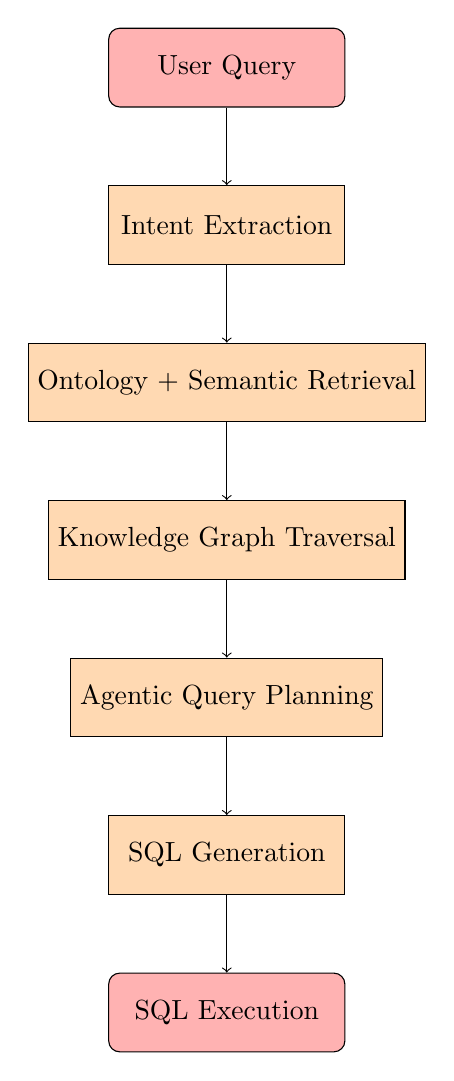
\begin{tikzpicture}[node distance=2cm]

\tikzstyle{startstop} =
[rectangle,
rounded corners,
minimum width=3cm,
minimum height=1cm,
text centered,
draw=black,
fill=red!30]

\tikzstyle{process} =
[rectangle,
minimum width=3cm,
minimum height=1cm,
text centered,
draw=black,
fill=orange!30]

\node (start) [startstop] {User Query};

\node (intent) [process, below of=start]
{Intent Extraction};

\node (retrieval) [process, below of=intent]
{Ontology + Semantic Retrieval};

\node (graph) [process, below of=retrieval]
{Knowledge Graph Traversal};

\node (planner) [process, below of=graph]
{Agentic Query Planning};

\node (generator) [process, below of=planner]
{SQL Generation};

\node (execution) [startstop, below of=generator]
{SQL Execution};

\draw[->] (start) -- (intent);
\draw[->] (intent) -- (retrieval);
\draw[->] (retrieval) -- (graph);
\draw[->] (graph) -- (planner);
\draw[->] (planner) -- (generator);
\draw[->] (generator) -- (execution);

\end{tikzpicture}
\begin{figure}[h]
    \centering
    \includegraphics[width=0.8\textwidth]{A1.png}
    \caption{System Architecture}
    \label{fig:architecture}
\end{figure}
\end{center}

\section{Design Philosophy}

The architecture is based on five major principles.

\subsection{Semantic Grounding}

Queries are grounded into business ontology concepts before SQL generation occurs.

\subsection{Structural Truth}

Neo4j graph traversal guarantees valid join discovery.

\subsection{Controlled Generation}

The LLM receives only filtered contextual schema information.

\subsection{Database Independence}

Ontology abstracts business meaning from physical schema implementations.

\subsection{Agentic Reasoning}

The architecture decomposes SQL generation into multiple reasoning stages.

\section{Info DB: Relational Metastore}

\subsection{Motivation}

Static JSON-based schema summaries are inefficient for large-scale enterprise databases. The system utilizes a dedicated \textbf{Info DB} (SQLite-based) as a high-performance relational metastore to manage schema metadata and data samples.

\subsection{Info DB Schema Model}

The Metastore consists of two primary tables:
\begin{itemize}
    \item \textbf{meta\_tables}: Stores canonical table names, view flags, primary key definitions, and JSON-serialized data samples.
    \item \textbf{meta\_columns}: Stores detailed column attributes including data types, nullability, and unique categorical sample values (e.g., list of Cities or Categories).
\end{itemize}

\subsection{Extraction Workflow}

The extraction is performed using the \textbf{SchemaExtractor} engine:
\begin{enumerate}
    \item \textbf{SQLAlchemy Inspection}: Dynamically reflects the target database schema.
    \item \textbf{Data Sampling}: Fetches the top 3-5 rows per table to provide context for the LLM.
    \item \textbf{Categorical Discovery}: Extracts unique values from low-cardinality columns to improve semantic filtering.
    \item \textbf{Relational Persistence}: Writes the processed metadata into the Info DB tables for granular retrieval.
\end{enumerate}


\begin{figure}[h]
    \centering
    \includegraphics[width=0.8\textwidth]{Talk_to_Data_archF.png}
    \caption{System Architecture}
    \label{fig:architecture}
\end{figure}
\section{Domain Ontology Layer}
\subsection{Purpose}

The ontology layer acts as a semantic bridge between:
\begin{center}
Human Language $\leftrightarrow$ Database Schema
\end{center}

\subsection{Ontology Components}

The ontology contains:
\begin{itemize}
    \item Business Concepts,
    \item Synonyms,
    \item Metric Definitions,
    \item Hierarchical Relationships,
    \item Business Rules,
    \item Derived Attributes.
\end{itemize}

\subsection{Ontology Example}

\begin{lstlisting}[language=json]
{
  "Customer": {
    "aliases": [
      "Client",
      "Buyer"
    ]
  },

  "Revenue": {
    "formula":
    "SUM(Orders.TotalAmount)"
  }
}
\end{lstlisting}

\subsection{Benefits}

The ontology layer:
\begin{itemize}
    \item Eliminates semantic ambiguity,
    \item Supports business vocabulary,
    \item Improves SQL generation accuracy,
    \item Enables cross-database compatibility.
\end{itemize}

\section{Domain \& Rule Processing}

\subsection{Catalogue Loader}

The architecture integrates a dynamic Catalogue Loader that processes JSON-based product catalogues (e.g., \texttt{field\_catalogue.json}). This component defines:
\begin{itemize}
    \item \textbf{Business Rules \& Formulas:} Calculations for metrics like profit margins, discounting, and net revenue.
    \item \textbf{Formatting Constraints:} Rules for decimal rounding, percentage scaling, and null handling.
    \item \textbf{Recursive Rules:} Table-level hierarchical processing rules for complex data structures.
\end{itemize}

\subsection{Ontology \& Rule Ingestion}

During the database synchronization phase, the system enriches the Neo4j Knowledge Graph with business logic:
\begin{itemize}
    \item \textbf{Rule Nodes:} Column-level and table-level recursive rules are ingested directly into the Knowledge Graph as \texttt{:Rule} and \texttt{:RecursiveRule} nodes, linked via \texttt{HAS\_RULE} and \texttt{HAS\_RECURSIVE\_RULE} relationships.
    \item \textbf{LLM Domain Ontologist:} An automated ontologist dynamically maps technical schema metadata to business concepts and synonyms, ingesting them as \texttt{:Concept} and \texttt{:Synonym} nodes.
\end{itemize}
This ensures that the Semantic Retrieval Layer and the Agentic Query Planner have immediate access to ground-truth business rules alongside structural metadata.

\section{Knowledge Graph Layer}

\subsection{Graph Representation}

The enterprise schema is modeled as a graph structure.

\subsection{Node Types}

\begin{itemize}
    \item Table,
    \item Column,
    \item Concept,
    \item Synonym,
    \item Metric,
    \item Constraint.
\end{itemize}

\subsection{Relationship Types}

\begin{itemize}
    \item HAS\_COLUMN,
    \item REFERENCES,
    \item MAPS\_TO,
    \item DERIVED\_FROM,
    \item BELONGS\_TO.
\end{itemize}

\subsection{Cypher Example}

\begin{lstlisting}[language=SQL]
CREATE (:Table {name:'Customers'})

CREATE (:Column {
    name:'CustomerID'
})

MATCH (t:Table {name:'Customers'}),
      (c:Column {name:'CustomerID'})
CREATE (t)-[:HAS_COLUMN]->(c)
\end{lstlisting}

\subsection{Join Path Discovery}

Neo4j identifies valid relational paths dynamically.

Example:
\begin{center}
Customers $\rightarrow$ Orders $\rightarrow$ OrderDetails $\rightarrow$ Products
\end{center}

This prevents invalid join hallucinations.

\section{Semantic Vector Retrieval}

\subsection{Motivation}

Users often express queries using vague or contextual business terminology.

Examples:
\begin{itemize}
    \item High value clients,
    \item Best selling products,
    \item Top performing regions.
\end{itemize}

\subsection{Embedding Pipeline}

The following objects are embedded:
\begin{itemize}
    \item Table descriptions,
    \item Column semantics,
    \item Business definitions,
    \item Metric descriptions,
    \item Historical query examples.
\end{itemize}

\subsection{Vector Storage}

Embeddings are stored in ChromaDB.

\subsection{Hybrid Retrieval}

The retrieval process combines:
\begin{enumerate}
    \item Ontological matching,
    \item Graph traversal,
    \item Vector similarity search.
\end{enumerate}

\section{Intent Extraction Engine}

\subsection{Purpose}

Intent extraction converts natural language into structured representations.

Example query:

\begin{quote}
Show top customers by revenue during 2023
\end{quote}

Extracted intent:

\begin{lstlisting}[language=json]
{
  "entity": "Customer",
  "metric": "Revenue",
  "time_period": "2023",
  "aggregation": "SUM",
  "ranking": "DESC"
}
\end{lstlisting}

\subsection{Hybrid Extraction Strategy}

The system combines:
\begin{itemize}
    \item Rule-based extraction,
    \item LLM structured extraction,
    \item Embedding similarity,
    \item Ontology expansion.
\end{itemize}

\section{Agentic Query Planning}

\subsection{Need for Planning}

Direct SQL generation is unreliable for large enterprise schemas.

Therefore, the system introduces an intermediate planning phase.

\subsection{Planning Tasks}

The planner determines:
\begin{itemize}
    \item Required tables,
    \item Join paths,
    \item Aggregations,
    \item Filters,
    \item Sorting,
    \item Grouping logic.
\end{itemize}

\subsection{Intermediate Plan}

\begin{lstlisting}[language=json]
{
  "tables": [
    "Customers",
    "Orders"
  ],

  "joins": [
    "Customers.CustomerID =
     Orders.CustomerID"
  ],

  "aggregations": [
    "SUM(Orders.TotalAmount)"
  ]
}
\end{lstlisting}

\section{Prompt Engineering \& LLM Constraints}

\subsection{Model Selection: gemma4:31b-cloud Provider:Ollama}

The system utilizes the \textbf{Gemma} model through the \textbf{Ollama Cloud} variant as the core reasoning engine. Gemma is selected due to its strong instruction-following capability, structured-output generation, and effectiveness in SQL synthesis tasks. Since the proposed system requires accurate interpretation of natural language queries, schema grounding, join-path reasoning, and SQL/Cypher generation, Gemma serves as the central LLM component in the agentic query execution pipeline.

In the proposed architecture, Gemma is accessed through Ollama Cloud rather than being executed entirely on local hardware. This allows the system to use larger cloud-hosted model variants for complex reasoning tasks while avoiding local GPU and memory constraints. However, cloud execution introduces usage limits that must be considered during system design, especially for repeated query execution, agentic retries, and self-correction workflows.

\subsection{Ollama Cloud Usage Metrics}

To evaluate the practical resource consumption of the selected cloud model, two query executions were tested using Ollama Cloud usage statistics. The first query was a complex multi-table analytical query involving customer ranking, discounted revenue calculation, supplier-country matching, shipping-country filtering, category aggregation, distinct supplier counting, and first qualifying order detection. The second query was a simple query with lower reasoning and schema traversal requirements.

The observed Ollama Cloud usage metrics are shown below:

\begin{table}[h]
\centering
\caption{Ollama Cloud Usage Increase by Query Complexity}
\begin{tabular}{|l|c|c|}
\hline
\textbf{Query Type} & \textbf{Session Usage Increase} & \textbf{Weekly Usage Increase} \\
\hline
Simple Query & 0.2\% & 0.1\% \\
\hline
Medium Query & 0.3\% & 0.1\% \\
\hline
Hard Query & 1.0\% & 0.4\% \\
\hline
Complex Query & 1.1\% & 0.4\% \\
\hline
\end{tabular}
\end{table}
Based on the observed values, the complex query consumed approximately \textbf{5.5 times more session quota} and \textbf{4 times more weekly quota} than the simple query. This demonstrates that query complexity has a direct impact on cloud resource consumption. Queries involving multiple joins, nested aggregations, ranking logic, semantic filtering, and self-correction attempts consume significantly more cloud quota than simple lookup or retrieval queries.

After the simple query execution, the remaining Ollama Cloud quota was:

\begin{table}[h]
\centering
\caption{Remaining Ollama Cloud Quota After Query Execution}
\begin{tabular}{|l|c|c|}
\hline
\textbf{Limit Type} & \textbf{Current Usage} & \textbf{Remaining Quota} \\
\hline
Session Usage & 23.2\% & 76.8\% \\
\hline
Weekly Usage & 8.6\% & 91.4\% \\
\hline
\end{tabular}
\end{table}

Using the measured per-query consumption, the approximate number of additional queries that can be executed is estimated as follows:

\begin{table}[h]
\centering
\caption{Approximate Query Capacity for Fresh Ollama Cloud Limits}
\resizebox{\textwidth}{!}{
\begin{tabular}{|l|c|c|c|c|}
\hline
\textbf{Query Type} & \textbf{Session Usage} & \textbf{Weekly Usage} & \textbf{Fresh Session Capacity} & \textbf{Fresh Weekly Capacity} \\
\hline
Simple & 0.2\% & 0.1\% & 500 & 1000 \\
\hline
Medium & 0.3\% & 0.1\% & 333 & 1000 \\
\hline
Hard & 1.0\% & 0.4\% & 100 & 250 \\
\hline
Complex & 1.1\% & 0.4\% & 90 & 250 \\
\hline
\end{tabular}
}
\end{table}

These metrics indicate that Ollama Cloud is suitable for the proposed system, but efficient context management and query complexity control are necessary to maintain scalability. In particular, complex enterprise queries and repeated agentic retries should be optimized to reduce unnecessary prompt expansion and cloud usage.

\subsection{Token Limitation and Cloud Usage Management}

The Gemma 4 cloud model provides a large context window capacity, with the cloud variant supporting up to \textbf{256K tokens}. However, large enterprise schemas, metadata catalogs, semantic graphs, sample records, historical query contexts, and agentic retry logs can still introduce scalability, latency, and cloud usage challenges when injected directly into prompts.

The observed Ollama Cloud metrics show that complex analytical queries consume significantly more quota than simple queries. Therefore, token limitation management is not only required for fitting within the context window, but also for reducing cloud usage, improving latency, and supporting repeated query execution within session and weekly limits.

To address this, the proposed architecture employs:

\begin{itemize}
    \item \textbf{Dynamic Context Filtering}: Only metadata and schema information relevant to the extracted intent are retrieved from the Info DB and injected into the prompt context. This reduces unnecessary token usage and avoids exposing the model to irrelevant tables or columns.
    
    \item \textbf{Semantic Context Selection}: Tables, columns, relationships, and sample records are filtered using semantic similarity and relationship-aware retrieval. This ensures that only the most relevant schema components are passed to the model.
    
    \item \textbf{Granular Summarization}: Large schema descriptions, sample rows, relationship metadata, and historical query examples are summarized and truncated based on semantic relevance and query complexity.
    
    \item \textbf{Graph-Aware Retrieval}: Relevant semantic graph and relationship graph substructures are selectively retrieved instead of loading the complete enterprise graph into the prompt. This allows the system to preserve join-path reasoning while minimizing prompt size.
    
    \item \textbf{Multi-Stage Chaining}: Query processing is decomposed into multiple stages such as:
    
    \[
    \text{Intent Extraction}
    \rightarrow
    \text{Semantic Mapping}
    \rightarrow
    \text{Query Planning}
    \rightarrow
    \text{SQL/Cypher Generation}
    \]
    
    This ensures that each stage operates within safe token boundaries while improving reasoning accuracy, reducing hallucinations, and preventing unnecessary cloud quota consumption.
    
    \item \textbf{Adaptive Prompt Injection}: Prompt size, schema depth, relationship depth, and retrieval breadth are dynamically adjusted based on query difficulty. Simple queries receive minimal context, while complex analytical queries receive richer schema and relationship context.
    
    \item \textbf{Quota-Aware Query Execution}: Since Ollama Cloud usage increases with query complexity, the system monitors query difficulty and retry count before invoking larger cloud model variants. Simple queries can be handled with smaller or lower-cost models, while complex queries and final correction steps can use larger Gemma cloud variants.
    
    \item \textbf{Retry Budget Control}: Agentic self-correction is limited using a retry budget. If SQL execution fails, only the error message, failed SQL, and relevant schema fragments are passed back to the model instead of reinjecting the entire context.
\end{itemize}

\subsection{Prompt Strategy}

Three distinct prompt types are used in the proposed system:

\begin{enumerate}
    \item \textbf{Strict Grounding Prompt}: Forces the LLM to use only the canonical table names, column names, relationships, and business definitions provided in the retrieved context. This reduces hallucinated schema references and improves SQL validity.
    
    \item \textbf{Chain-of-Thought Planning}: Encourages the model to reason through intent, entity mapping, join paths, filtering conditions, aggregation logic, and ranking requirements before generating the final SQL/Cypher query. In implementation, only the final structured plan or query is retained to reduce unnecessary token usage.
    
    \item \textbf{Self-Correction Prompt}: If execution fails, the database error message, failed query, and relevant schema subset are fed back to the model for an agentic retry. This allows the system to repair syntax errors, incorrect joins, missing columns, or invalid aggregation logic without restarting the entire pipeline.
\end{enumerate}

The prompt strategy is designed to balance reasoning accuracy with cloud efficiency. The measured Ollama Cloud metrics show that complex queries consume substantially more quota than simple queries; therefore, the system avoids full-context prompting and instead uses adaptive, retrieval-based prompt construction for scalable enterprise query execution.
\section{SQL Generation Pipeline}

\subsection{Generation Inputs}

The SQL generator receives:
\begin{itemize}
    \item Ontology mappings,
    \item Verified joins,
    \item Semantic context from Info DB,
    \item Structured plans.
\end{itemize}

\subsection{Generated SQL Example}

\begin{lstlisting}[language=SQL]
SELECT
    c.CompanyName,
    SUM(o.TotalAmount) AS Revenue
FROM Customers c
JOIN Orders o
ON c.CustomerID = o.CustomerID
GROUP BY c.CompanyName
ORDER BY Revenue DESC
LIMIT 10;
\end{lstlisting}

\section{Validation Pipeline}

Generated SQL is validated using:
\begin{enumerate}
    \item Syntax verification,
    \item Schema validation,
    \item Permission checks,
    \item Join verification,
    \item Cost analysis.
\end{enumerate}

\subsection{Safety Controls}

The system blocks:
\begin{itemize}
    \item DELETE statements,
    \item UPDATE operations,
    \item Unauthorized access,
    \item Full table scans,
    \item Dangerous procedural execution.
\end{itemize}

\section{Programmatic Workflow}

\subsection{Phase 1: Synchronization}

\begin{enumerate}
    \item Database schema extraction,
    \item \textbf{Info DB persistence},
    \item Ontology generation,
    \item Graph ingestion,
    \item Embedding generation,
    \item Semantic indexing.
\end{enumerate}

\subsection{Phase 2: Retrieval}

\begin{enumerate}
    \item Intent extraction,
    \item Ontology mapping,
    \item Graph traversal,
    \item \textbf{Relational Metadata Retrieval (Info DB)},
    \item Query planning,
    \item SQL synthesis,
    \item Validation,
    \item Execution.
\end{enumerate}
\section{Prompt Evaluation}

The generated prompts were evaluated based on different query complexity levels. 
Each prompt was tested to analyze:
\begin{itemize}
    \item Semantic understanding
    \item Query generation accuracy
    \item Relationship reasoning capability
    \item Hallucination reduction
\end{itemize}

%------------------------------------------------

\subsection{Easy Level Prompt}

\subsubsection*{Prompt}

Show me the top 5 most expensive products with their colors

\vspace{0.5cm}

\subsubsection*{Output}

\begin{figure}[h]
    \centering
    \includegraphics[width=0.9\textwidth]{easy.png}
    \caption{Output for Easy Level Prompt}
\end{figure}

\newpage

%------------------------------------------------

\subsection{Medium Level Prompt}

\subsubsection*{Prompt}

List all customers who live in London and have placed at least one order.

\vspace{0.5cm}

\subsubsection*{Output}

\begin{figure}[h]
    \centering
    \includegraphics[width=0.9\textwidth]{medium.png}
    \caption{Output for Medium Level Prompt}
\end{figure}

\newpage

%------------------------------------------------

\subsection{Hard Level Prompt}

\subsubsection*{Prompt}

Which product categories have generated more than 20,000 in total sales?
Show the category name and the total revenue.


\vspace{0.5cm}

\subsubsection*{Output}

\begin{figure}[h]
    \centering
    \includegraphics[width=0.9\textwidth]{hard.png}
    \caption{Output for Hard Level Prompt}
\end{figure}

\newpage

%------------------------------------------------

\subsection{Extreme Level Prompt}

\subsubsection*{Prompt}

List the top 3 customers who have spent the most on products with a 'Black' color, and for each customer, show their primary city and the name of the very first 'Road Bike' they ever purchased.


\vspace{0.5cm}

\subsubsection*{Output}

\begin{figure}[h]
    \centering
    \includegraphics[width=0.9\textwidth]{extreme.png}
    \caption{Output for Extreme Level Prompt}
\end{figure}

\newpage
\section{Scalability Considerations}

The architecture supports:
\begin{itemize}
    \item PostgreSQL,
    \item MySQL,
    \item Oracle,
    \item SQL Server,
    \item Snowflake,
    \item SAP HANA.
\end{itemize}

\subsection{Distributed Scaling}

Future scaling mechanisms include:
\begin{itemize}
    \item Distributed vector search,
    \item Federated graph retrieval,
    \item Multi-agent orchestration,
    \item Streaming semantic indexing.
\end{itemize}

\section{Research Contributions}

The architecture contributes:
\begin{enumerate}
    \item Ontology-driven semantic abstraction,
    \item \textbf{Info DB relational metadata management},
    \item Graph-constrained SQL generation,
    \item Hybrid graph-vector retrieval,
    \item Enterprise semantic grounding.
\end{enumerate}

\section{Future Scope}

Potential future enhancements include:
\begin{itemize}
    \item Self-evolving ontologies,
    \item Reinforcement learning from query feedback,
    \item Autonomous optimization agents,
    \item Cross-enterprise semantic interoperability,
    \item Explainable query generation systems.
\end{itemize}

\section{Conclusion}

The proposed architecture introduces a robust enterprise-grade semantic retrieval framework that integrates ontology reasoning, graph traversal, vector semantics, and agentic SQL generation.

By decoupling business language from physical database schemas through a **hybrid Info DB and Graph architecture**, the system enables scalable, context-aware, and structurally valid natural language querying across complex enterprise environments.

The fusion of:
\begin{itemize}
    \item Knowledge Graph reasoning,
    \item Info DB Relational Metastore,
    \item Semantic embeddings,
    \item Agentic planning
\end{itemize}

creates a highly extensible foundation for next-generation enterprise data intelligence systems.

\end{document}
